\newchapstyle
\chapter{Tips for operating the EBPGs at the TU Delft Kavli Nanolab}
\label{app:ebeam}
%% Start the actual chapter on a new page.
\afterpage{\pagecolor{none}}\newpage

\section{Height adjustment}\label{sec:height}
%
When mounting chips on the EBPG sample holder, the chip needs to be held in place by clamps, while the holder height, tilt and rotation can be adjusted using micrometer screws.
%
Naturally, the substrate never ends up completely horizontal due to manual errors, but in addition to surface tilt, bending also occurs regularly:
%
Clamping the chip down with the holder clamps leads to tension and bending of the chip of up to several micrometers per mm, see Fig.~\ref{fig:heightmap}.
%
These height differences can lead to distortions or stitching in the exposed pattern if not accounted for: 
%
The electron beam is focused only at one height. 
%
If height measurement is deactivated in cjob, the EBPG will not adjust the focus and patterns exposed this way can exhibit gaps reminiscent of stitching errors, or become overexposed.
%
For this reason, activating beam height adjustment should be standard practice and can lead to significant improvements in patterning quality.

\begin{figure}
	\centering
	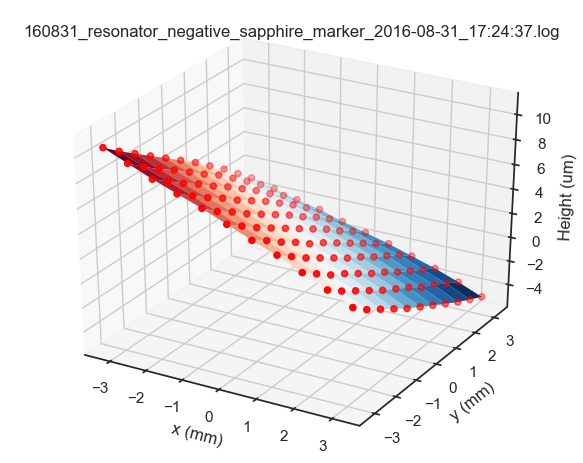
\includegraphics[width=0.3\linewidth]{{appendix/figs/160831_resonator_negative_sapphire_marker_2016-08-31_17_24_37.log3D}.png}
	\hfill
	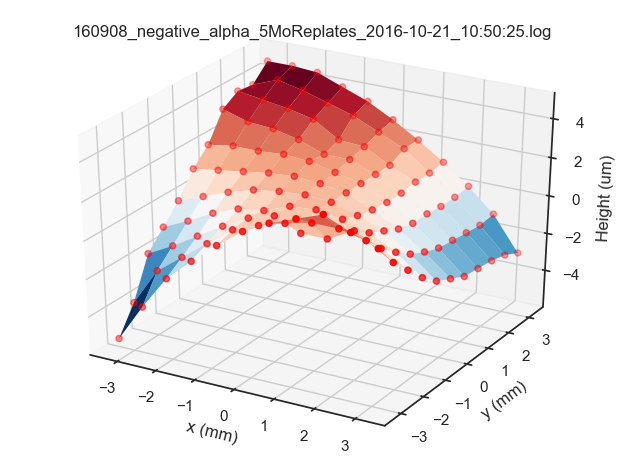
\includegraphics[width=0.3\linewidth]{{appendix/figs/160908_negative_alpha_5MoReplates_2016-10-21_10_50_25.log3D}.png}
	\hfill
	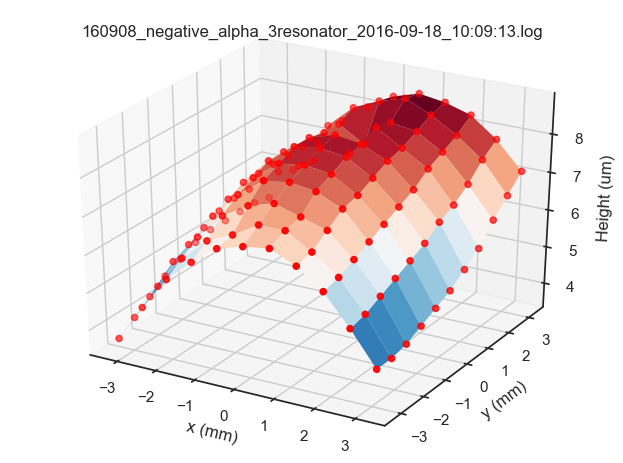
\includegraphics[width=0.3\linewidth]{{appendix/figs/160908_negative_alpha_3resonator_2016-09-18_10_09_13.log3D}.png}	
	\\
	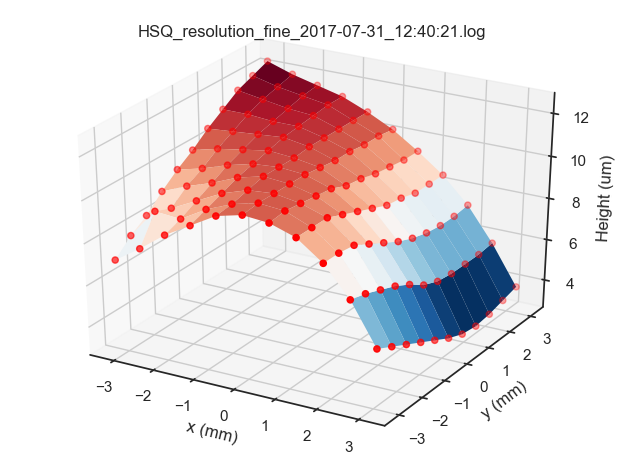
\includegraphics[width=0.3\linewidth]{{appendix/figs/HSQ_resolution_fine_2017-07-31_12_40_21.log3D}.png}
	\hfill
	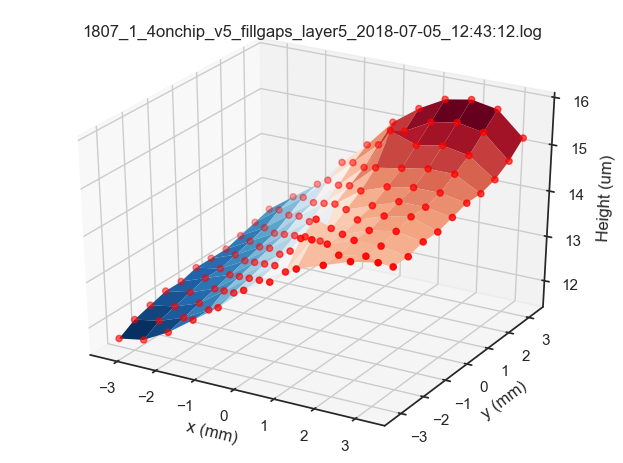
\includegraphics[width=0.3\linewidth]{{appendix/figs/1807_1_4onchip_v5_fillgaps_layer5_2018-07-05_12_43_12.log3D}.png}	
	\hfill
	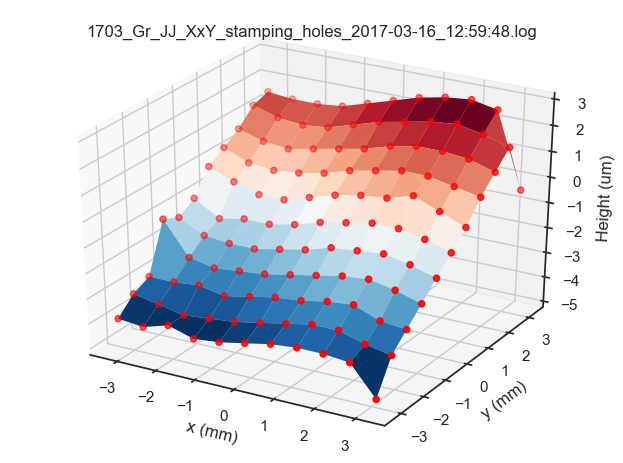
\includegraphics[width=0.3\linewidth]{{appendix/figs/1703_Gr_JJ_XxY_stamping_holes_2017-03-16_12_59_48.log3D}.png}
	\\
	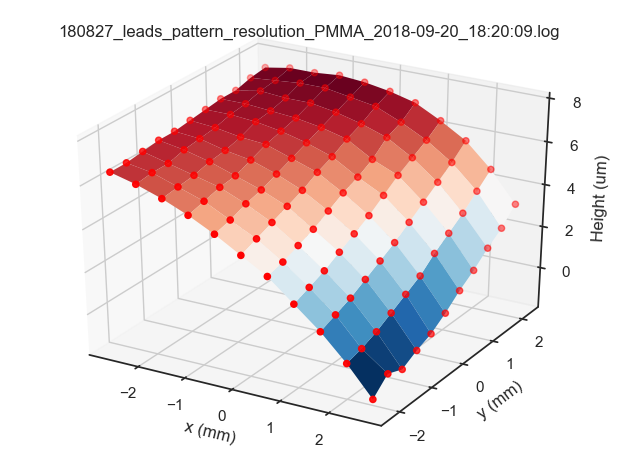
\includegraphics[width=0.3\linewidth]{{appendix/figs/180827_leads_pattern_resolution_PMMA_2018-09-20_18_20_09.log3D}.png}
	\hfill
	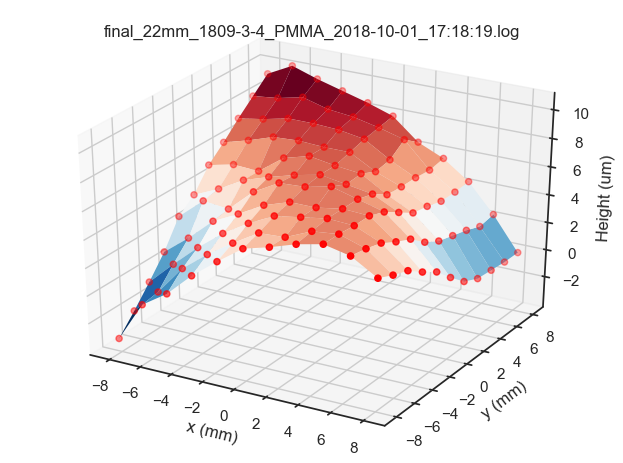
\includegraphics[width=0.3\linewidth]{{appendix/figs/final_22mm_1809-3-4_PMMA_2018-10-01_17_18_19.log3D}.png}
	\hfill
	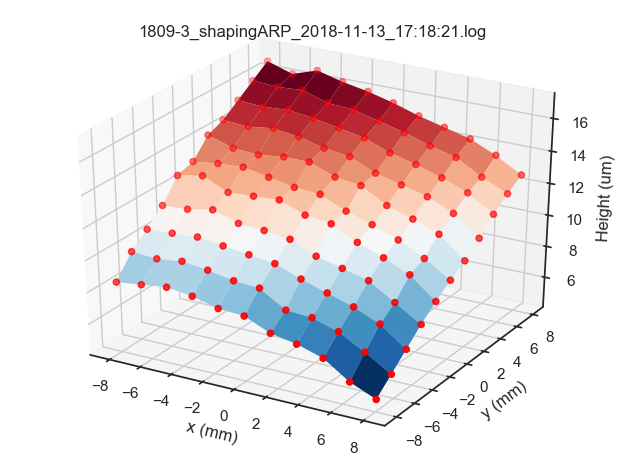
\includegraphics[width=0.3\linewidth]{{appendix/figs/1809-3_shapingARP_2018-11-13_17_18_21.log3D}.png}
	\caption{
		\textbf{A selection of heightmaps of different samples and different substrates, exposed on the EBPG 5000+ and the EBPG 5200.}
		%
		Sample heights are aligned with three height screws with which tilt can be adjusted for.
		%
		Substrate bending can be due to the clamps holding the chip in place.
	}
	\label{fig:heightmap}
\end{figure}


\section{Stitching errors}

We occasionally encountered stitching errors in our patterns, especially on the EBPG5000+, as shown in Fig.~\ref{fig:stitching}.
%
These defects manifest themselves as cuts or offsets at the main field borders, between parts of the pattern written by the ebeam.
%
Each part of a pattern within a main field, approximately \SI{700x700}{\micro\meter}, will be exposed without any stage movement or height adjustment.
%
Stitching errors thus usually occur at the borders between main fields.
%
Aside from the beam being out of focus, as discussed above, these can also be due to unusually large drifts over time in the piezoelectronics of the EBPG.
%
To minimize the risk of encountering these issues, the following points should always be checked when setting up a job file:
%
\begin{description}
	\item[Height measurements]
	%
	To eliminate errors due to the beam being out of focus, enable automatic height adjustment in cjob.
	%
	Note that the job will fail if the measured height is out of range.
	\item[Exposure time]
	%
	Minimizing exposure time can reduce the susceptibility to drift errors.
	%
	Techniques to consider are to change to a bigger beam, or to switch pattern polarity, e.g. by switching between a negative and a positive resist, or patterning with lift-off versus dry-etching.
	%
	\item[Main field placement]
	%
	Choosing the main field placement such that the most critical parts of a pattern are not crossing main field borders can limit the effect of stitching.
	%
	This can be achieved e.g. by changing the mainfield size to a more a suitable value, choosing \textit{floating} main field placement, and selecting \textit{follow geometry} as writing order.
	%
	\item[Separate exposures]
	%
	Stitching-sensitive parts of a pattern can be split off from those that are less susceptible to stitching errors, and be exposed separately within one job.
	%
	For example, the holey ground used in superconducting microwave circuits for flux trapping should be split off from the coplanar waveguides, since CPWs should not have stitching errors, while defects in the ground plane are not critical.
\end{description}

\begin{figure}
	\centering
	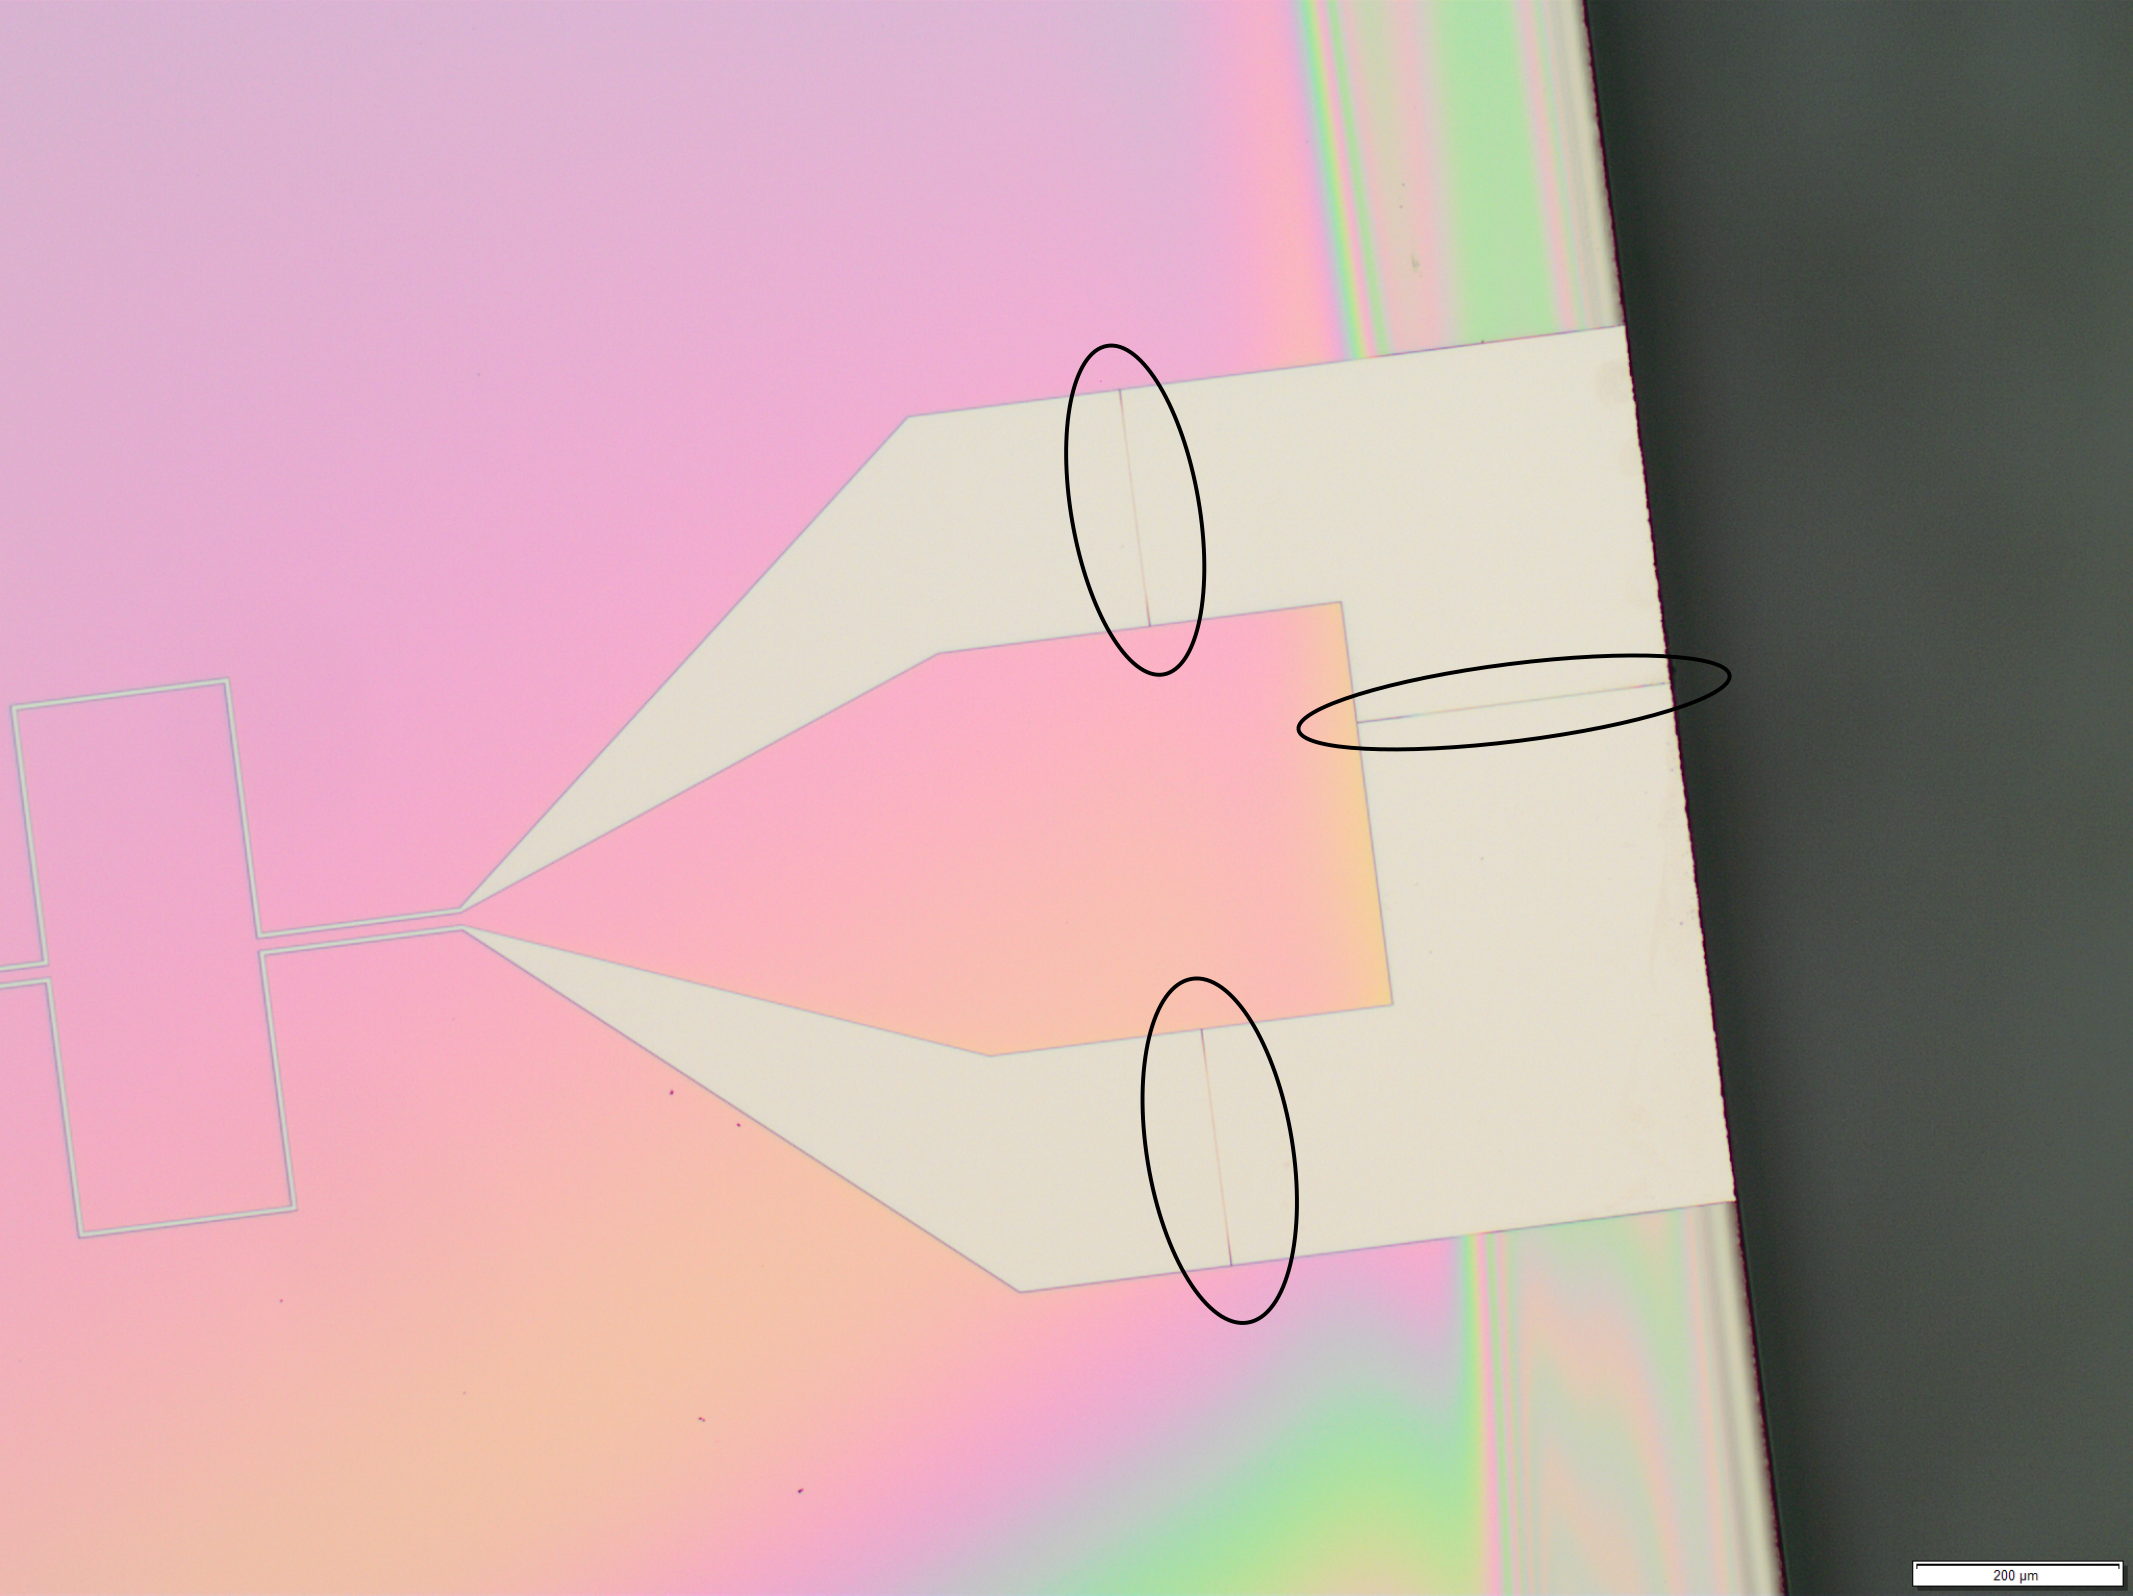
\includegraphics[width=0.3\linewidth]{{appendix/figs/stitching/Image_2019.svg}.png}
	\hfill
	\includegraphics[width=0.3\linewidth]{{appendix/figs/stitching/Image_21071.svg}.png}
	\hfill
	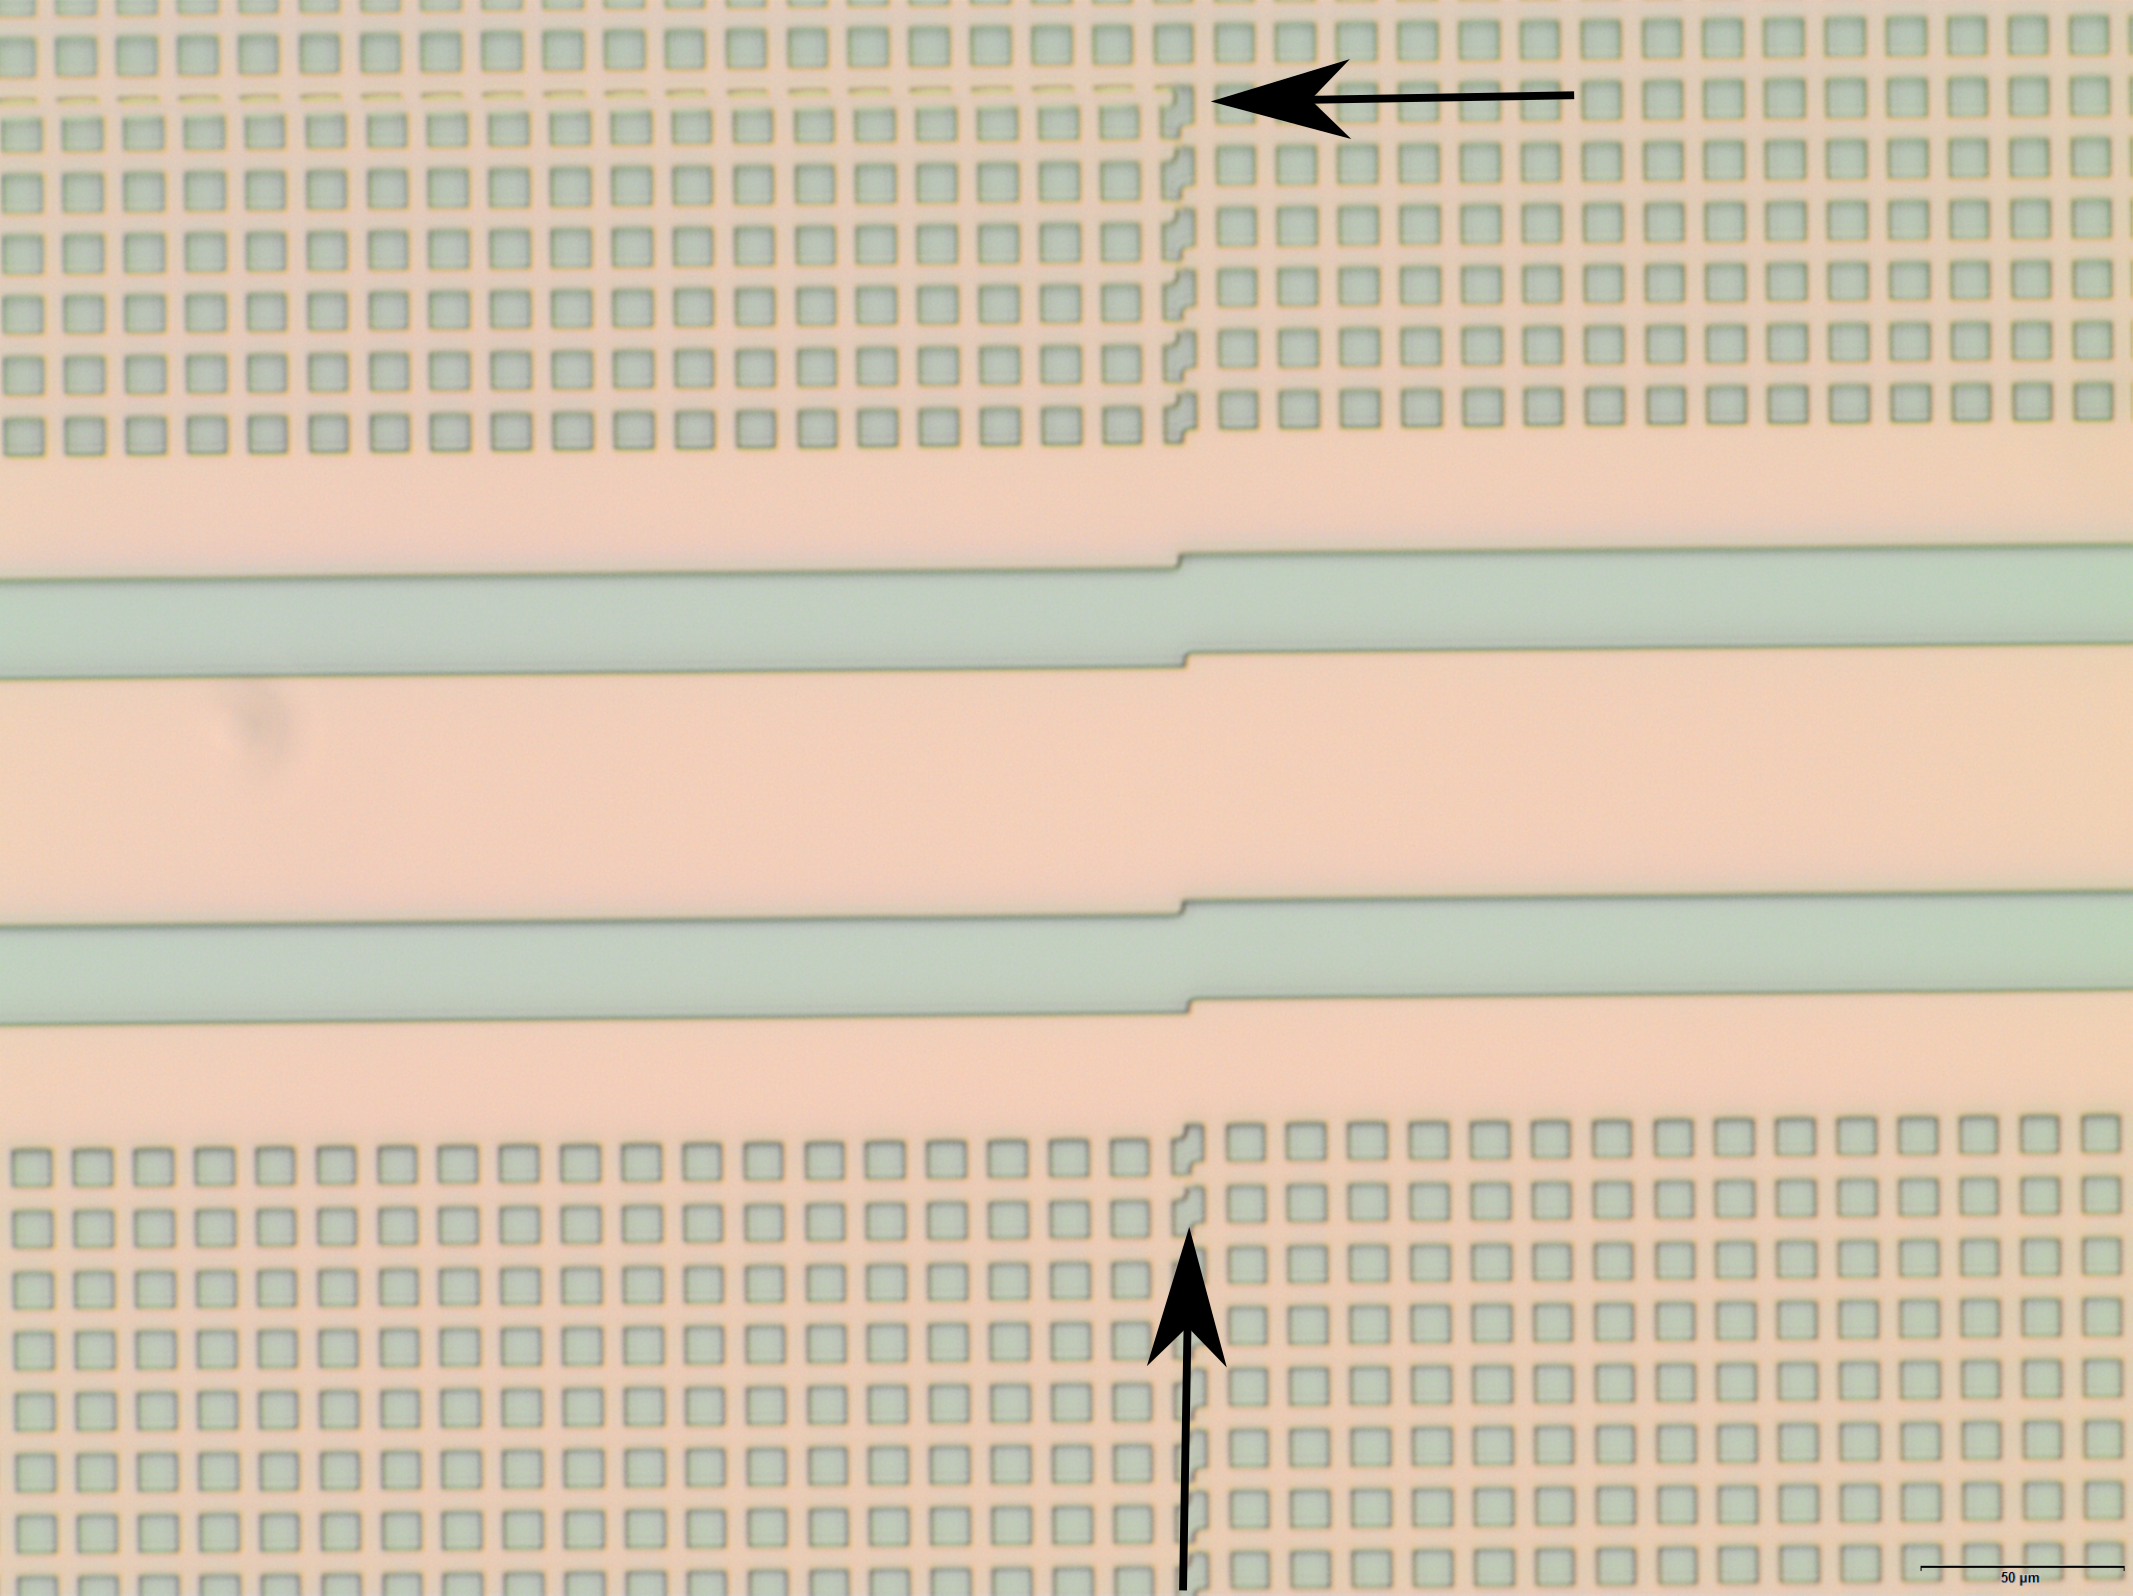
\includegraphics[width=0.3\linewidth]{{appendix/figs/stitching/Image_21825.svg}.png}	
	\caption{
		\textbf{Stitching errors encountered on the EBPG5000+.}
		%
		Parts of the pattern are unexposed (left, as marked by the black ellipsoids) or offset from each other (center and right, marked by ellipsoids and arrows), leading to severe defects in the circuit pattern.
	}
	\label{fig:stitching}
\end{figure}

\section{Ebeam alignment}
Here, we provide information, tips and tricks on how ebeam alignment works and how to implement it reliably on the Raith EBPG 5000+ and 5200 in the TU Delft Kavli cleanroom.
%
This is important because when writing patterns onto a chip, you will need to specify the location of where on the chip you want your pattern to be.
%
In the case of single-layer exposure, you can simply note down the coordinates of two opposite corners of your chip, from which you can calculate the chip center.
%
This point can then be forwarded to the EBPG as location for the exposure.

\subsection{Alignment of various layers to each other}
It is good practice to add alignment marks to your pattern in case you will want to do another ebeam step on your sample. 
%
Note that even combining ebeam and photolithography steps are possible is suitable markers are chosen.
%
Obviously, for multiple steps you will want to have a very good alignment of the individual steps with respect to the previous layers. 
%
There are various types of ebeam markers available in cjob. 
%
In our group we usually make use of rectangular markers that are \SI{20x20}{\micro\meter}. 
%
Depending on the polarity, i.e. whether these will be elevated (positive) or holes (negative), these markers are called RP20 or RN20, respectively.
%
Depending on how good your alignment needs to be you might do with just one set of markers

\subsubsection{How marker search works}
There are two ways for searching for and aligning to markers:
\begin{enumerate}
	\item Manually: 
	%
	This is only possible in \lstinline|operator| mode: 
	%
	Move to the marker positions (e.g. via \lstinline|almic2ebpg| or directly via \lstinline|mpos|, turn on the SEM and align to the markers. 
	%
	This way you can align to any recognizable structure with known position. 
	%
	You should only use this if the machine cannot recognize your markers, e.g. due to dirt on top.
	%
	\item Automatically: 
	%
	This method should be used preferably because the EBPG's software algorithm is much better than a human.
	%
	In your cjob file you need to tell the ebeam which marker type (RECT for rectangular metallic, TOPO for topographic makers), POSitive or NEGative tone and what size they are. 
	%
	Rectangular markers can have lengths ranging from \SIrange{20}{100}{\micro\meter}.
\end{enumerate}

The default markers, as they are on the sample holders, are \lstinline|RECT POS 20,20|, or \lstinline|RP20|.
%

For an automatic marker search, the EBPG starts at the specified position and scans outwards in a rectangular spiral, while at the same time measuring the contrast. 
%
In the end, once it measures a step of significant contrast and length that matches the specified marker type, it will stop. 
%
If it doesn't find anything, it will abort after a certain radius.
%
The marker search parameters are:
\begin{itemize}
	\item expected contrast \lstinline|CONTRA| (default \SI{97}{\percent})
	\item maximum radius \lstinline|ISRAD| (default \SI{50}{\micro\meter}, at most half a scan field)
	\item step \lstinline|ISXSTP, ISYSTP| (default \SI{30}{\percent} marker size)
\end{itemize}
 
\subsubsection{General rules for good alignment}

Note that you should keep a free area (recommended are >\SI{100x100}{\micro\meter}) around each marker.
%
This will help to avoid search failures due to confusion with other features. 
%
Also note that your markers should not be too close to your patterns, since marker search exposes the sample at a very high dose.

At least three markers are needed for correcting rotation, shift and scaling. 
%
However, it is recommended to use four markers to also account for shear and perspective distortion because the SEM detector is placed at an angle, which can lead to image distortions.

For most precise alignment (specs of the EBPG5000 and 5200 are below \SI{10}{\nano\meter}) these steps should be followed:
%
\begin{itemize}
	\item Do not use manual marker search.
	%
	The EBPG is usually better than a human.
	%
	\item Never use markers twice. 
	%
	Especially small beams can be extremely sensitive to any dirt on your markers, so make sure you have enough backup markers (at least one set per step).
	%
	Scanning markers during alignmnt leads to contamination from carbon deposition, potentially rendering them useless for future steps.
	%
	\item Do both rough and fine alignment: 
	%
	Do one alignment on R20 at the exposure level, one R20 alignment at the layout level, and one R10 alignment at the pattern level
	%
	\item Use small markers for fine alignment (i.e. RN10/RP10 as the last alignment step)
	%
	\item Put all patterns to be exposed inside the area enclosed by the markers.
	%
	\item The pattern should be within \SI{500}{\micro\meter} of each marker, meaning markers should not be spaced further apart than \SI{1}{\milli\meter} from each other.
\end{itemize}

\subsubsection{Rough alignment}
\begin{itemize}
	\item If the EBPG cannot find your markers, you might consider manual marker search (set marker type to \lstinline|JOY| and run job as \lstinline|operator|). 
	%
	Alignment will be significantly worse in this case, but at least you might be able to expose
	%
	\item Dirt on your markers can lead to the EBPG not recognizing them or, worse, misinterpreting edges, so that your pattern will be scaled or even misaligned.
	%
	\item For alignment down to approximately \SI{1}{\micro\meter}, it is not necessary to put all of your pattern inside an area enclosed by your markers. 
	%
	For a \SI{10x10}{\milli\meter} chip, you can for example place your markers at $\pm$\SI{3000}{\micro\meter}, $\pm$\SI{4000}{\micro\meter} and still expose and align all the way to the outside of the chip edge (with worse alignment the further outside the marker area you expose)
\end{itemize}

\subsection{Example workflow of high-accuracy alignment on a large chip}
%
This is an example workflow from Felix' device \textit{1809.3} exposed on 14 November 2018 at 17:04:55.
%
The pattern to be exposed is located on a \SI{22x22}{\milli\meter} chip, further divided into four \SI{10x10}{\milli\meter} chips, each with three DC bias cavities. 
%
At the end of two of each cavities per chip, there is a graphene JJ with several ebeam steps, which require high-accuracy alignment to each other. 
%
As an example we will cover the alignment for the third exposure, \textit{shapingARP}. 
%
Note that every single pattern is different from the others, so we cannot simply use the same patterns for each junction, but require individual patterns, hence the large number of patterns and colors, cf. Fig.~\ref{fig:ebeam1}.

\begin{figure}
	\centering
	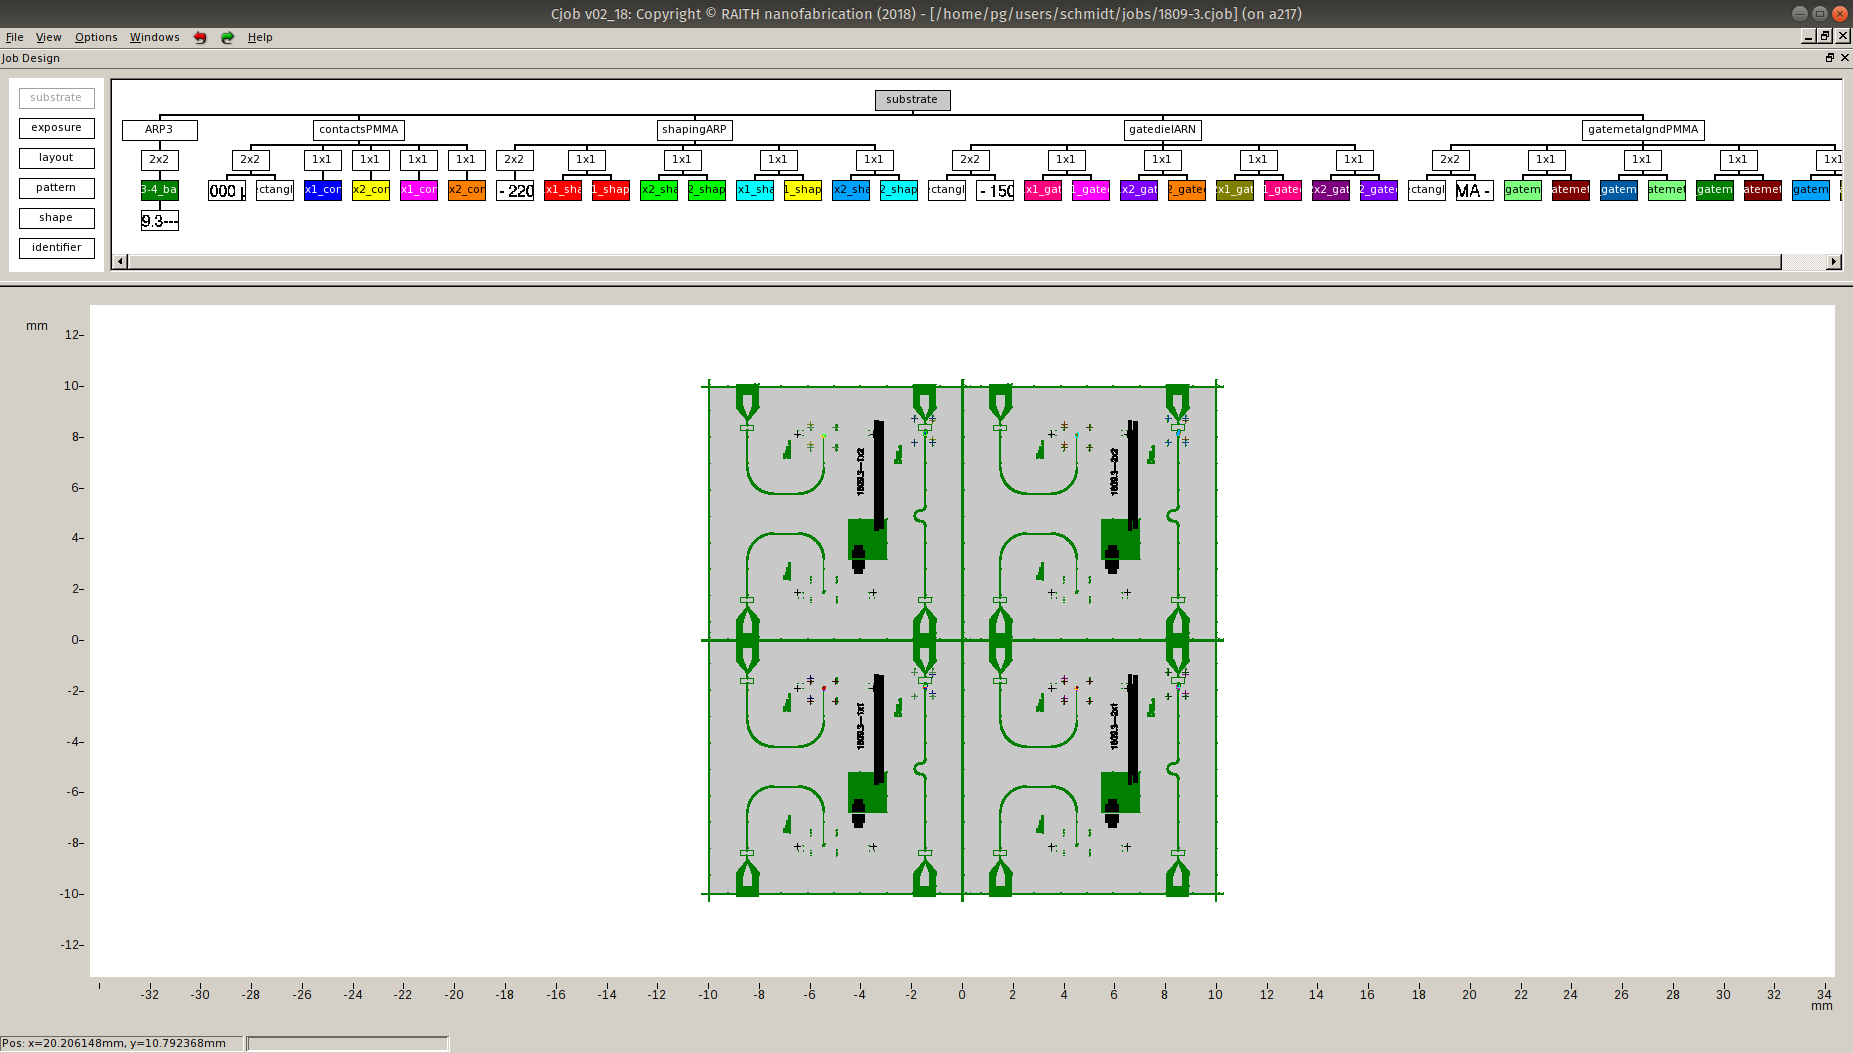
\includegraphics[width=\linewidth]{appendix/figs/ebeam1}
	\caption{
	\textbf{Cjob file for device 1809.3}
	}
	\label{fig:ebeam1}
\end{figure}


\subsubsection{First step: Alignment at the exposure level}
%
Since we have several chips on the big one, we will first get the mapping of the entire large chip. 
%
For this, we find the four outermost markers, which in this case is RN20 at ($\pm$6500,$\pm$8100), cf. Fig.~\ref{fig:ebeam2}.

\begin{figure}
	\centering
	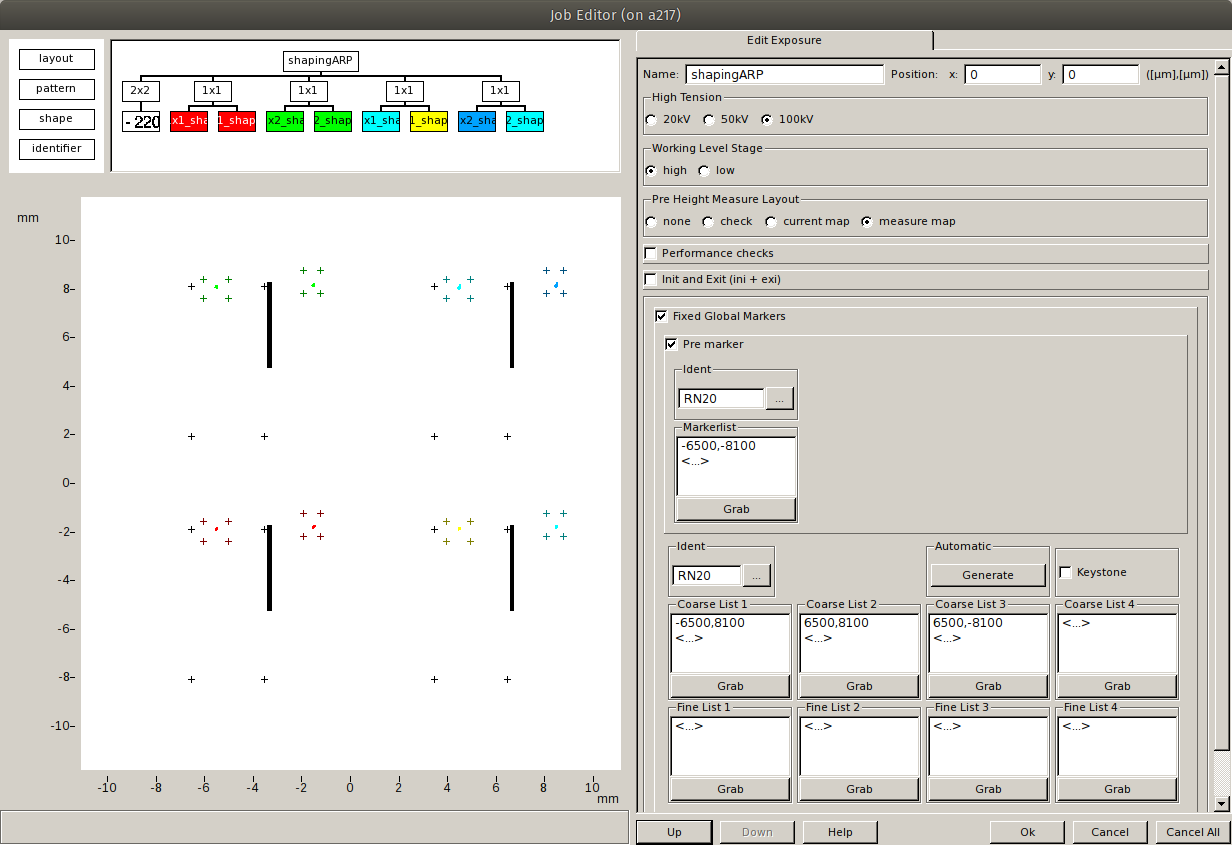
\includegraphics[width=\linewidth]{appendix/figs/ebeam2}
	\caption{\textbf{First step: Alignment at the exposure level}}
	\label{fig:ebeam2}
\end{figure}

\subsubsection{Second step: Alignment at the layout level}
%
Now that we have the general orientation of our large chip, we go into each of the four sub-chips and align the beam to four chip-markers. 
%
For the bottom-left chip, this is for example RN20 at (-6500,-8100), (-6500,-1900), (-3500,-1900), (-3500,-8100), cf. Fig.~\ref{fig:ebeam3}.
%
Note that we also use keystone correction here.

\begin{figure}
	\centering
	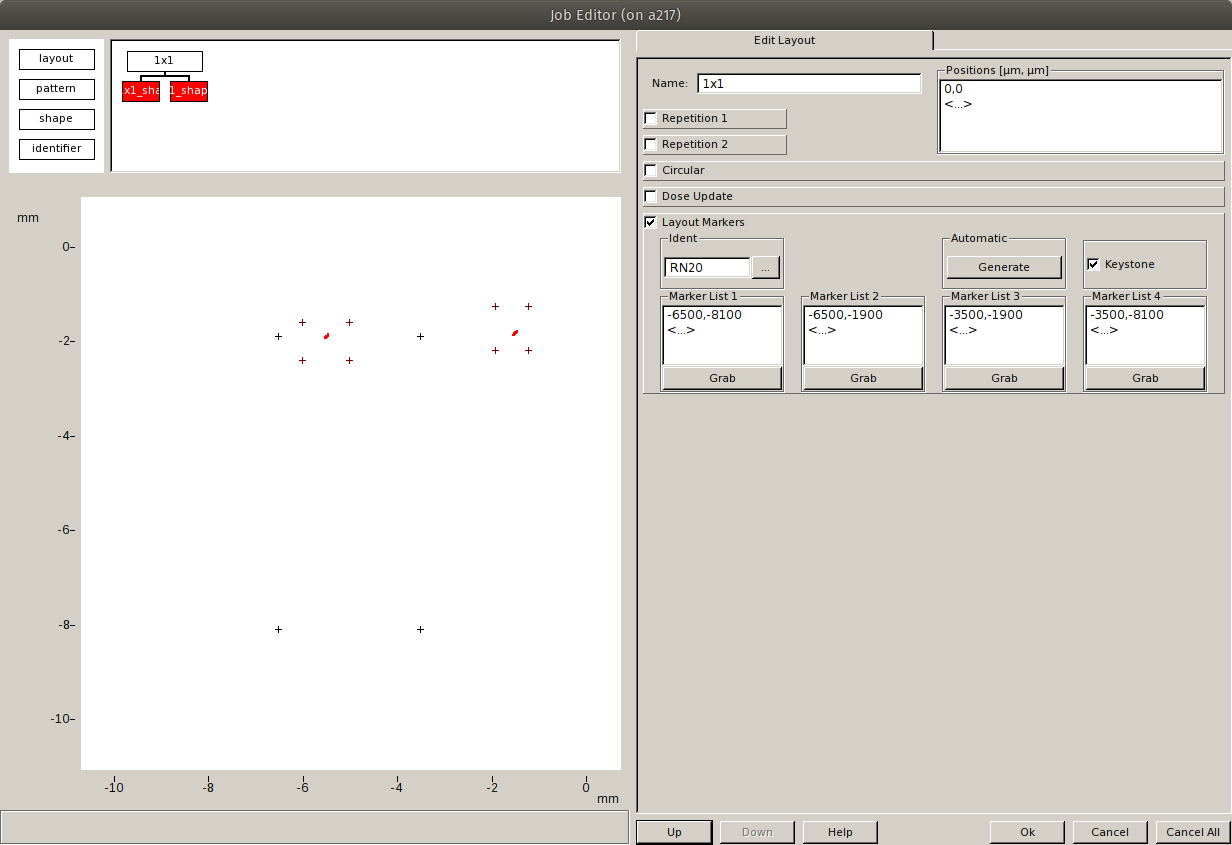
\includegraphics[width=\linewidth]{appendix/figs/ebeam3}
	\caption{\textbf{Second step: Alignment at the layout level}}
	\label{fig:ebeam3}
\end{figure}

\subsubsection{Third step: Alignment at the pattern level}
%
On each chip we will do two exposures with different patterns for two bias cavities. 
%
Since the patterns are spaced far apart, we choose to do a separate alignment for each exposure with very closely spaced markers. 
%
We now also switch to RN10 markers, since these are smaller and therefore the marker search is less likely to expose too much resist around our sample. 
%
Here for example the marker group of RN10 is (-1900,-2200), (-1200,-2200), (-1200,-1250), (-1900,-1250), cf. Fig.~\ref{fig:ebeam4}.
%
The xdistance between two markers is \SI{700}{\micro\meter}, the ydistance \SI{950}{\micro\meter}. 
%
Note that we also use keystone correction here.

\begin{figure}
	\centering
	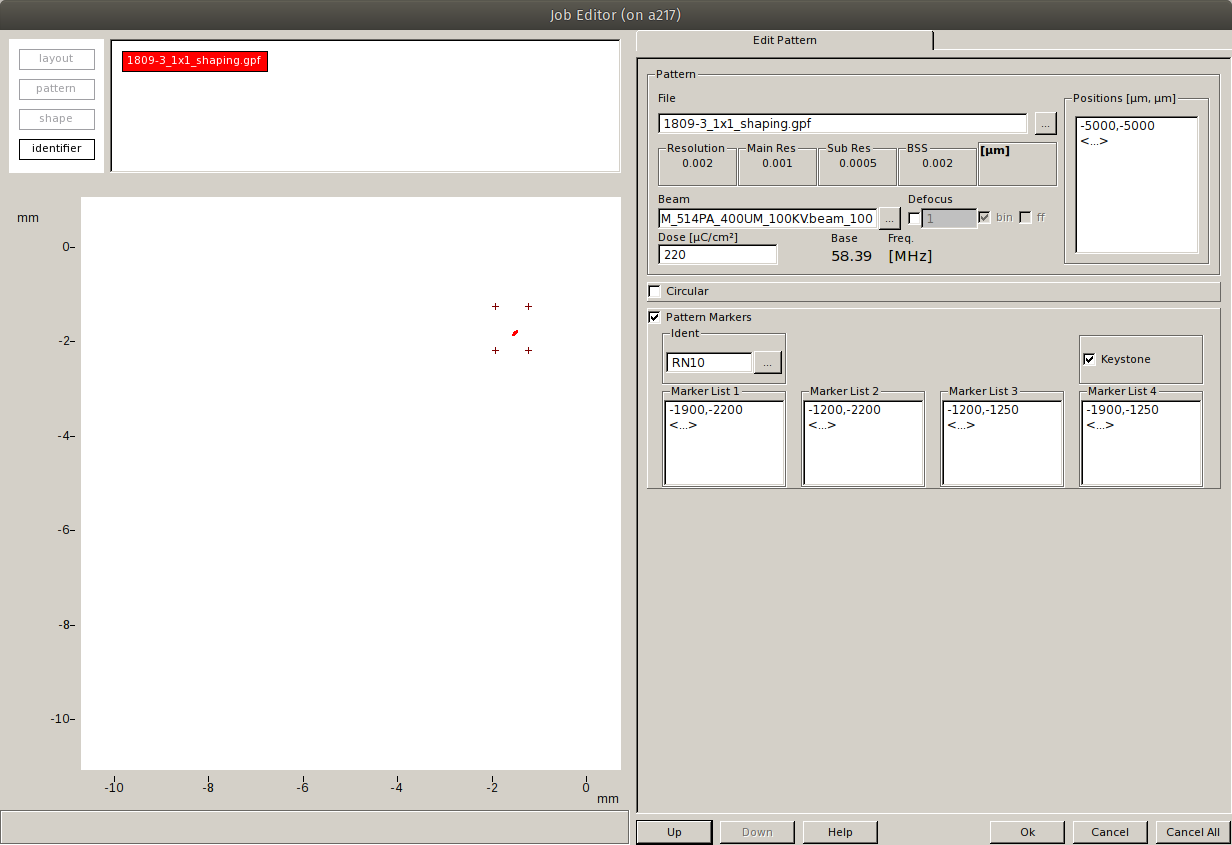
\includegraphics[width=\linewidth]{appendix/figs/ebeam4}
	\caption{\textbf{Third step: Alignment at the pattern level}}
	\label{fig:ebeam4}
\end{figure}


\subsubsection{How did the job go?}
Let's take a look at the log file, located on the ebpg5200 under \texttt{pg/users/schmidt/log/}, filename \texttt{1809-3\_shapingARP\_2018-11-14\_170455.log}.
%
Marker search starts in line 1831:
%
\lstinputlisting[firstline=1831,lastline=1842,firstnumber=1831,numbers=left]{appendix/1809-3_shapingARP_2018-11-14_170455.log}
%
Clearly, there was some misalignment between the actual marker position and the one specified for the job (\SI{10}{\micro\meter} in x, \SI{0.3}{\micro\meter} in y).
%
Note that the EBPG already compensates for the measured sample height at the marker (l.~1838) (see also Sec.~\ref{sec:height}).
%
Next, the marker search continues with the other three markers (ll.~1875-1909):
%
\lstinputlisting[firstline=1875,lastline=1909,firstnumber=1875,numbers=left]{appendix/1809-3_shapingARP_2018-11-14_170455.log}
%
We can see that the EBPG found all three markers, but it detected significant shifts:
\begin{itemize}
	\item Marker 1 was found at -6522.129, 8099.725 versus at -6500.000, 8100.000 (\SI{22.1}{\micro\meter}, \SI{0.3}{\micro\meter})
	\item Marker 2 was found at 6477.666, 8117.098 versus at 6500.000, 8100.000 (\SI{22.3}{\micro\meter},\SI{17.1}{\micro\meter})
	\item Marker 3 was found found at 6499.656, -8083.052 versus at 6500.000, -8100.000 (\SI{0.3}{\micro\meter}, \SI{16.9}{\micro\meter})
\end{itemize}
This implies nonnegligible scaling and rotation.
%
Good thing we did marker search! 
%
These shifts can be reduced if you do the rotation alignment very precise. 
%
I seemed to have been a bit sloppy here, but the EBPG can still account for this without any problems.

The EBPG then continues with searching the markers in the second step, at the layout patterns (ll.~2744-2801):
%
\lstinputlisting[firstline=2744,lastline=2801,firstnumber=2744,numbers=left]{appendix/1809-3_shapingARP_2018-11-14_170455.log}
%
Obviously, the first alignment on the exposure level was already quite good, since we now already have alignment precision to our marker positions on the sub-micron level.~
%
This is good enough for most cases, but not for multi-step patterns at with submicron dimension which require very precise feature alignment, in this case below \SI{100}{\nano\meter}.

As a last step, we search for the RN10 markers at the pattern level (ll.~2840-2895):
%
\lstinputlisting[firstline=2840,lastline=2895,firstnumber=2840,numbers=left]{appendix/1809-3_shapingARP_2018-11-14_170455.log}
%
At this stage, the misalignment is below \SI{100}{\nano\meter} for each marker. 
%
This is sufficient and the EBPG continues by exposing the pattern.


%\clearpage
%\references{dissertation}

